\documentclass{article}
\usepackage{ijcai16}
\usepackage{times}
\usepackage{multirow}
\usepackage{latexsym}
\usepackage{mathrsfs}
\usepackage{graphicx}
\usepackage{subfig}
\usepackage{amsfonts}
\usepackage{amssymb}
\usepackage{amsmath}
\usepackage{bm}
\usepackage{url}
\usepackage{tikz-dependency}
\usepackage{pgfplots}
\usepackage{xcolor}
\usepackage{array}

\allowdisplaybreaks

\newenvironment{itemize*}%
  {\begin{itemize}%
    \setlength{\itemsep}{0pt}%
    \setlength{\parskip}{0pt}}%
  {\end{itemize}}
  \newenvironment{enumerate*}%
  {\begin{enumerate}%
    \setlength{\itemsep}{0pt}%
    \setlength{\parskip}{0pt}}%
  {\end{enumerate}}


\newcommand{\tabincell}[2]{\begin{tabular}{@{}#1@{}}#2\end{tabular}}
\pgfplotsset{compat=1.5}
%\setlength\titlebox{6.5cm}  % Expanding the titlebox
\DeclareMathOperator*{\argmax}{arg\,max}
\DeclareMathOperator*{\MOD}{MOD}

%\newcommand{\tabincell}[2]{\begin{tabular}{@{}#1@{}}#2\end{tabular}}

%\newcommand  \citet[1]{\newcite{#1}}
\newcommand\newcite[1]{\citeauthor{#1} [\citeyear{#1}]}

\def\W{\mathbf{W}}
\def\U{\mathbf{U}}
\def\bb{\mathbf{b}}

\def\V{\mathbf{V}}
\def\e{\mathbf{e}}
\def\h{\mathbf{h}}
\def\rr{\mathbf{r}}
\def\bx{\mathbf{x}}
\def\by{\mathbf{y}}
\def\cc{\mathbf{c}}
\def\ii{\mathbf{i}}
\def\ff{\mathbf{f}}
\def\oo{\mathbf{o}}
\def\u{\mathbf{u}}
\def\g{\mathbf{g}}
\def\p{\mathbf{p}}
\def\q{\mathbf{q}}
\def\bt{\mathbf{t}}
\def\SS{\mathbf{S}}
\def\ss{\mathbf{s}}
\def\cc{\mathbf{c}}
\def\bw{\mathbf{w}}
\def\H{\mathbf{H}}
\def\P{\mathbf{P}}
\def\R{\mathbb{R}}
\def\l{\mathbf{l}}
%Chinese Package
%\usepackage[slantfont,boldfont]{xeCJK} % 允许斜体和粗体
%\setmainfont[Mapping=tex-text]{Times New Roman} % 使用 XeTeX 的 text-mapping 方案,正确显示 LaTeX 样式的双引号(`` '')
%\setCJKmainfont{SimSun}
%\usetikzlibrary{positioning,bayesnet}
%\title{Clockwork Memory Neural Network for Modelling \\ Sentences and Documents}%\Thanks{}
%\title{Neural Matching Model By Jointly Learning to \\ Align and Match}
\title{Modelling Interaction of Sentence Pair with Coupled-LSTMs}

\author{Pengfei Liu \quad Xipeng Qiu\thanks{Corresponding author.} \quad Xuanjing Huang\\
Shanghai Key Laboratory of Intelligent Information Processing, Fudan University\\
School of Computer Science, Fudan University\\
825 Zhangheng Road, Shanghai, China\\
\{pfliu14,xpqiu,xjhuang\}@fudan.edu.cn}



\date{}

\begin{document}
\maketitle
%\quote
\begin{abstract}
Recently, there is rising interest in modelling the interactions of two sentences with deep neural networks. However, most of the existing methods encode two sequences with separate encoders, in which a sentence is encoded with little or no information from the other sentence. In this paper, we propose a deep architecture to model the strong  interaction of sentence pair with two coupled-LSTMs. Specifically, we introduce two coupled ways to model the interdependences of two LSTMs, coupling the local contextualized interactions of two sentences. We then aggregate these interactions and use a dynamic pooling to select the most informative features. Experiments on two very large datasets demonstrate the efficacy of our proposed architecture and its superiority to state-of-the-art methods.
\end{abstract}
%\quote



\section{Introduction}

Distributed representations of words or sentences have been widely used in many natural language processing (NLP) tasks, such as text classification \cite{kalchbrenner2014convolutional}, question answering and machine translation \cite{sutskever2014sequence} and so on.
Among these tasks, a common problem is modelling the relevance/similarity of the sentence pair, which is also called text semantic matching.

Recently, deep learning based models is rising a substantial interest in text semantic matching and have achieved some great progresses~\cite{hu2014convolutional,qiu2015convolutional,wan2015deep}.

 %A good representation of the variable-length text should fully capture the semantics of natural language.



According to the phases of interaction between two sentences, previous models can be classified into three categories.

%several neural network based models were proposed to model the interaction of the sentence pair at different phase.
\vspace{-1em}
\paragraph{Weak interaction Models}
Some early works focus on sentence level interactions, such as ARC-I\cite{hu2014convolutional}, CNTN\cite{qiu2015convolutional} and so on. These models first encode two sequences with some basic (Neural Bag-of-words, BOW) or advanced (RNN, CNN) components of neural networks separately, and then compute the matching score based on the distributed vectors of two sentences. In this paradigm, two sentences have no interaction until arriving final phase.
\vspace{-1em}
\paragraph{Semi-interaction Models}
Some improved methods focus on utilizing multi-granularity representation (word, phrase and sentence level), such as  MultiGranCNN \cite{yin2015convolutional} and Multi-Perspective CNN \cite{he2015multi}.
Another kind of models use soft attention mechanism to obtain the representation of one sentence by  depending on representation of another sentence, such as  ABCNN \cite{yin2015abcnn}, Attention LSTM\cite{rocktaschel2015reasoning,hermann2015teaching}.
These models can alleviate the weak interaction problem, but are still insufficient to model the contextualized interaction on the word as well as phrase level.
\vspace{-1em}
\paragraph{Strong Interaction Models}
These models directly build an interaction space between two sentences and model the interaction at different positions. ARC-II \cite{hu2014convolutional} and MV-LSTM \cite{wan2015deep}. These models enable the model to easily capture the difference between semantic capacity of two sentences.


 %Matching is of central importance to natural language processing. In fact, many problems in natural language processing can be formalized as matching between two short texts, with different matching relations in different applications. For example, in paraphrase identification the relation is synonymy, and in information retrieval it is relevance. In the meantime matching is also a challenging problem, since it requires modeling of the two short texts as well as their relation.

%\begin{figure}[t]\centering
%  \includegraphics[width=0.80\linewidth]{./fig/fig_intro.png}
%  \caption{Four Architectures}\label{fig:rnn}
%\end{figure}

%\begin{figure}[t]\centering
%  \subfloat[\tiny Parallel LSTMs]{
%        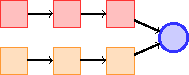
\includegraphics[width=0.4\linewidth]{./standalone/intro-1.pdf}
%  }\hspace{0.2cm}
%  \subfloat[\tiny Attentive LSTMs]{
%        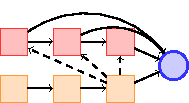
\includegraphics[width=0.4\linewidth]{./standalone/intro-2.pdf}
%  }\\
%  \subfloat[\tiny Tight-coupled-LSTMs]{
%        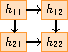
\includegraphics[width=0.4\linewidth,height=2cm]{./standalone/intro-3.pdf}
%  }\hspace{0.2cm}
%  \subfloat[\tiny Tight-coupled-LSTMs]{
%        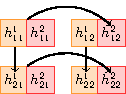
\includegraphics[width=0.4\linewidth]{./standalone/intro-4.pdf}
%  }
%  \caption{Four architectures to model sentence pair.}\label{fig:arc-4}
%\end{figure}



 In this paper, we propose a new deep neural network architecture to model the strong interactions of two sentences.
 Different with modelling two sentences with separated LSTMs, we utilize two interdependent LSTMs, called coupled-LSTMs, to fully affect each other at different time steps. The output of coupled-LSTMs at each step depends on both sentences. Specifically, we propose two interdependent ways for the coupled-LSTMs: loosely coupled model (LC-LSTMs) and tightly coupled model (TC-LSTMs). Similar to bidirectional LSTM for single sentence \cite{schuster1997bidirectional,graves2005framewise}, there are four directions can be used in coupled-LSTMs. To utilize all the information of four directions of coupled-LSTMs, we aggregate them and adopt a dynamic pooling strategy to automatically select the most informative interaction signals. Finally, we feed them into a fully connected layer, followed by an output layer to compute the matching score.

 The contributions of this paper can be summarized as follows.
 \begin{enumerate}
   \item Different with the architectures of using similarity matrix, our proposed architecture directly model the strong interactions of two sentences with coupled-LSTMs, which can capture the useful local semantic relevances of two sentences. Our architecture can also capture the multiple granular interactions by several stacked coupled-LSTMs layers.
   \item Compared to the previous works on text matching, we perform extensive empirical studies on two very large datasets. The massive scale of the datasets allows us to train a very deep neural networks. Experiment results demonstrate that our proposed architecture is more effective than state-of-the-art methods.
 \end{enumerate}

\section{Sentence Modelling with LSTM}

%Long short-term memory network (LSTM) can map the input sequence of arbitrary length to a fixed-sized vector, and has been successfully applied to a wide range of NLP tasks, such as machine translation \cite{sutskever2014sequence}, language modeling \cite{sutskever2011generating} and text matching \cite{rocktaschel2015reasoning}.

Long short-term memory network (LSTM)~\cite{hochreiter1997long} is a type of recurrent neural network (RNN) \cite{Elman:1990}, and
specifically addresses the issue of learning long-term dependencies. LSTM maintains a memory cell that updates and exposes its content only when deemed necessary.

%A number of minor modifications to the standard LSTM unit have been made.
While there are numerous LSTM variants, here we use the LSTM architecture used by \cite{jozefowicz2015empirical}, which is similar to the architecture of \cite{graves2013generating} but without peep-hole connections.

We define the LSTM \emph{units} at each time step $t$ to be a collection of vectors in $\mathbb{R}^d$: an \emph{input gate} $\ii_t$, a \emph{forget gate} $\ff_t$,  an \emph{output gate} $\oo_t$, a \emph{memory cell} $\cc_t$ and a hidden state $\h_t$. $d$ is the number of the LSTM units. The elements of the gating vectors $\ii_t$, $\ff_t$ and $\oo_t$ are in $[0, 1]$.

The LSTM is precisely specified as follows.

\begin{align}
	\begin{bmatrix}
		\mathbf{\tilde{c}}_{t} \\
		\mathbf{o}_{t} \\
		\mathbf{i}_{t} \\
		\mathbf{f}_{t}
	\end{bmatrix}
	&=
	\begin{bmatrix}
		\tanh \\
		\sigma \\
		\sigma \\
		\sigma
	\end{bmatrix}
	T_{\mathbf{A},\mathbf{b}}
	\begin{bmatrix}
		\mathbf{x}_{t} \\
		\mathbf{h}_{t-1}
	\end{bmatrix},\label{eq:lstm1}\\
\mathbf{c}_{t} &=
		\mathbf{\tilde{c}}_{t} \odot \mathbf{i}_{t}
		+ \mathbf{c}_{t-1} \odot \mathbf{f}_{t}, \\
	\mathbf{h}_{t} &= \mathbf{o}_{t}  \odot \tanh\left( \mathbf{c}_{t}  \right)\label{eq:lstm2},
\end{align}
where $\bx_t$ is the input at the current time step;
$T_{\mathbf{A},\mathbf{b}}$ is an affine transformation which depends on parameters of the network $\mathbf{A}$ and $\mathbf{b}$.
$\sigma$ denotes the logistic sigmoid function and $\odot$ denotes elementwise multiplication. Intuitively, the forget gate controls the amount of which each unit of the memory cell is erased, the input gate controls how much each unit is updated, and the output gate controls the exposure of the internal memory state.

The update of each LSTM unit can be written precisely as follows
\begin{align}
(\h_t,\cc_t) &= \mathbf{LSTM}(\h_{t-1},\cc_{t-1},\mathbf{x}_t).
\end{align}
Here, the function $\mathbf{LSTM}(\cdot, \cdot, \cdot)$ is a shorthand for Eq. (\ref{eq:lstm1}-\ref{eq:lstm2}).

\section{Coupled-LSTMs for Strong Sentence Interaction}

To deal with two sentences, one straightforward method is to model them with two separate LSTMs. However, this method is difficult to model local interactions of two sentences. An improved way is to introduce attention mechanism, which has been used in many tasks, such as machine translation~\cite{bahdanau2014neural} and question answering~\cite{hermann2015teaching}.

Inspired by the multi-dimensional recurrent neural network \cite{graves2007multi,graves2009offline,byeon2015scene} and grid LSTM~\cite{kalchbrenner2015grid} in computer vision community, we propose two models to capture the interdependences between two parallel LSTMs, called \textbf{coupled-LSTMs} (C-LSTMs).
%\begin{enumerate}
%  \item The first architecture is similar to the 2-dimensional LSTM, which consider the different interactive way between two sequences. Strong Coupled Models
%  \item The second architecture is an improved version of attentive model.
%\end{enumerate}
\begin{figure}[t]\centering
\subfloat[Parallel LSTMs]{
        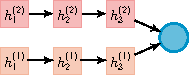
\includegraphics[width=0.4\linewidth]{./standalone/intro-1-u.pdf}\label{fig:arc-p}
  }\hspace{0.2cm}
  \subfloat[Attention LSTMs]{
        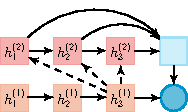
\includegraphics[width=0.4\linewidth]{./standalone/intro-2-u.pdf}\label{fig:arc-a}
  }\\
  \subfloat[Loosely coupled-LSTMs]{
  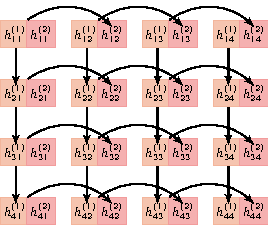
\includegraphics[width=0.50\linewidth]{./standalone/SLMD-8.pdf}\label{fig:arc-lc}
  }
  \hspace{0.2cm}
  \subfloat[Tightly coupled-LSTMs]{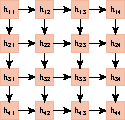
\includegraphics[width=0.41\linewidth]{./standalone/SLMD-7.pdf}\label{fig:arc-tc}
  }
  \caption{Four different coupled-LSTMs.}\label{fig:arc}
\end{figure}

To facilitate our models, we firstly give some definitions. Given two sequences $X = x_1,x_2,\cdots,x_n$ and $Y = y_1,y_2,\cdots,y_m$, we let $\bx_i \in \R^d$ denote the embedded representation of the word $x_i$. The standard LSTM have one temporal dimension. When dealing with a sentence, LSTM regards the position as time step. At position $i$ of sentence $x_{1:n}$, the output $\h_i$ reflects the meaning of subsequence $x_{0:i}={x_0,\cdots,x_i}$.

To model the interaction of two sentences as early as possible, we define $\h_{i,j}$ to represent the interaction of the subsequences $x_{0:i}$ and $y_{0:j}$.

Figure \ref{fig:arc}(c) and \ref{fig:arc}(d) illustrate our two propose models. For intuitive comparison of weak interaction parallel LSTMs, we also give  parallel LSTMs and attention LSTMs in Figure \ref{fig:arc}(a) and \ref{fig:arc}(b).

We describe our two proposed models as follows.


\subsection{Loosely Coupled-LSTMs (LC-LSTMs)}
To model the local contextual interactions of two sentences, we enable two LSTMs to be interdependent at different positions. Inspired by Grid LSTM~\cite{kalchbrenner2015grid} and word-by-word attention LSTMs \cite{rocktaschel2015reasoning}, we propose a loosely coupling model for two interdependent LSTMs.

More concretely, we refer to $\h_{i,j}^{(1)}$ as the encoding of subsequence $x_{0:i}$ in the first LSTM influenced by the output of the second LSTM on subsequence $y_{0:j}$. Meanwhile, $\h_{i,j}^{(2)}$ is the encoding of subsequence $y_{0:j}$ in the second LSTM influenced by the output of the first LSTM on subsequence $x_{0:i}$

$\h_{i,j}^{(1)}$ and $\h_{i,j}^{(2)}$ are computed as
\begin{align}
\h_{i,j}^{(1)} &= \mathbf{LSTM}^{1}(\mathbf{H}_{i-1}^{(1)},\cc_{i-1,j}^{(1)},\mathbf{\bx}_{i}), \\
\h_{i,j}^{(2)} &= \mathbf{LSTM}^{2}(\mathbf{H}_{j-1}^{(2)},\cc_{i,j-1}^{(2)},\mathbf{y}_{j}),
\end{align}
where
\begin{align}
\mathbf{H}_{i-1}^{(1)} = [\h_{i-1,j}^{(1)},\h_{i-1,j}^{(2)}], \\
\mathbf{H}_{j-1}^{(2)} = [\h_{i,j-1}^{(1)},\h_{i,j-1}^{(2)}].
\end{align}


\subsection{Tightly Coupled-LSTMs (TC-LSTMs)}

The hidden states of LC-LSTMs are the combination of the hidden states of two interdependent LSTMs, whose memory cells are separated. Inspired by the configuration of the multi-dimensional LSTM~\cite{byeon2015scene}, we further conflate both the hidden states and the memory cells of two LSTMs. We assume that $\h_{i,j}$ directly model the interaction of the subsequences $x_{0:i}$ and $y_{0:j}$, which depends on two previous interaction $\h_{i-1,j}$ and $\h_{i,j-1}$, where $i,j$ are the positions in sentence $X$ and $Y$.

We define a tightly coupled-LSTMs \emph{units} as follows.

\begin{align}
	\begin{bmatrix}
		\mathbf{\tilde{c}}_{i,j} \\
		\mathbf{o}_{i,j} \\
		\mathbf{i}_{i,j} \\
		\mathbf{f}_{i,j}^1 \\
		\mathbf{f}_{i,j}^2
	\end{bmatrix}
	&=
	\begin{bmatrix}
		\tanh \\
		\sigma \\
		\sigma \\
		\sigma \\
		\sigma
	\end{bmatrix}
	T_{\mathbf{A},\mathbf{b}}
	\begin{bmatrix}
		\mathbf{x}_{i} \\
        \mathbf{y}_{j} \\
		\mathbf{h}_{i,j - 1} \\
		\mathbf{h}_{i - 1,j}
	\end{bmatrix},\\
	\mathbf{c}_{i,j} &=
		\mathbf{\tilde{c}}_{i,j} \odot \mathbf{i}_{i,j}
		  + [\mathbf{c}_{i,j - 1},\mathbf{c}_{i - 1,j}]^\mathrm{T}
            \begin{bmatrix}
				\mathbf{f}_{i,j}^1 \\
				\mathbf{f}_{i,j}^2 \\
			\end{bmatrix} \\
	\mathbf{h}_{i,j} &= \mathbf{o}_{t}  \odot \tanh\left( \mathbf{c}_{i,j} \right)
\end{align}
where the gating units $\mathbf{i}_{i,j}$ and $\mathbf{o}_{i,j}$
determine which memory units are affected by the inputs through $\mathbf{\tilde{c}}_{i,j}$, and which memory cells are written to the hidden units $\mathbf{h}_{i,j}$.
$T_{\mathbf{A},\mathbf{b}}$ is an affine transformation which depends on parameters of the network $\mathbf{A}$ and $\mathbf{b}$.
In contrast to the standard LSTM defined over time, each memory unit $\cc_{i,j}$ of a tightly coupled-LSTMs has two preceding states
$\mathbf{c}_{i,j-1}$ and $\mathbf{c}_{i-1,j}$ and two corresponding forget gates $\mathbf{f}_{i,j}^1$ and $\mathbf{f}_{i,j}^2$.

%The entries of the gating vectors $\ii_{i,j}$, $\ff^1_{i,j}$, $\ff^2_{i,j}$ and $\oo_{i,j}$ are in $[0, 1]$.

\begin{figure*}[t]\centering
  %\includegraphics[width=0.9\linewidth]{./fig/2d-lstm-archi.png}
  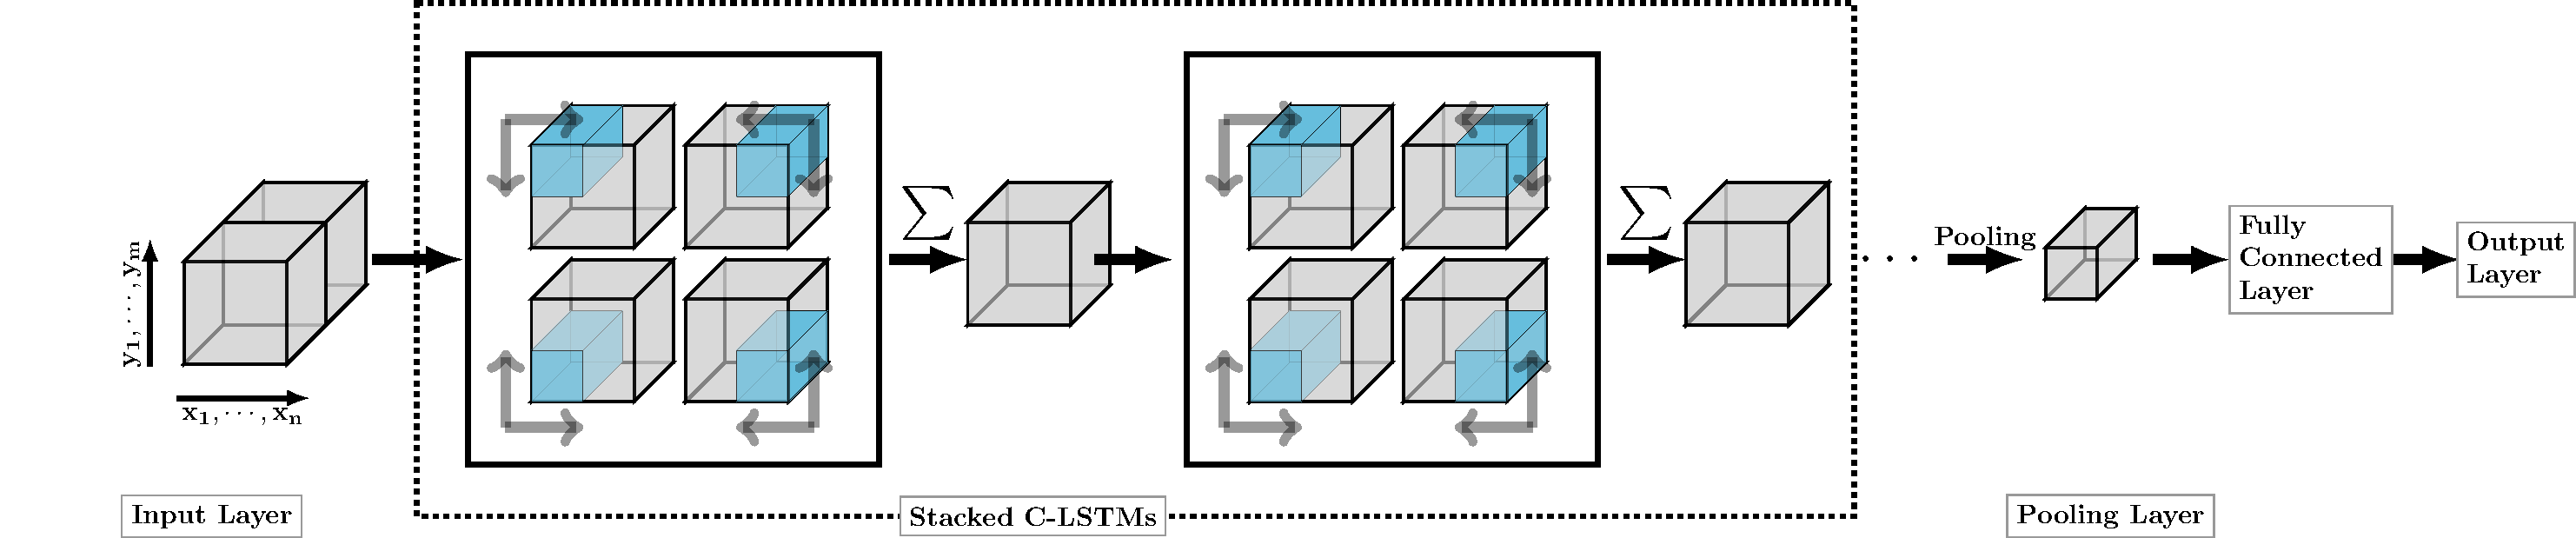
\includegraphics[width=1\linewidth]{./standalone/cubic-8.pdf}

  \caption{Architecture of coupled-LSTMs for sentence-pair encoding. Inputs are fed to four C-LSTMs followed by an aggregation layer. Blue cuboids represent different contextual information from four directions.}\label{fig:arc-4}
\end{figure*}



\subsection{Analysis of Two Proposed Models}
Our two proposed coupled-LSTMs can be formulated as
\small{
\begin{align}
(\h_{i,j},\cc_{i,j}) &= \textbf{C-LSTMs}(\h_{i-1,j},\h_{i,j-1},\cc_{i-1,j},\cc_{i,j-1},\bx_i,\by_j),
\end{align}
}
where $\textbf{C-LSTMs}$ can be either $\textbf{TC-LSTMs}$ or  $\textbf{LC-LSTMs}$.



 The input consisted of two type of information at step $(i,j)$ in coupled-LSTMs: temporal dimension
$\h_{i-1,j}, \h_{i,j-1}, \cc_{i-1,j}, \cc_{i,j-1}$ and depth dimension
$\mathbf{x}_i,\mathbf{y}_j$. The difference between TC-LSTMs and LC-LSTMs is the dependence of information from temporal and depth dimension.

%Each state in TC-LSTMs depend on all these information of the previous states, while each LSTM in loosely coupled model just uses its own internal memory and one input in depth dimension. Thus, TC-LSTMs can model  more strong interactions than LC-LSTMs.

\paragraph{Interaction Between Temporal Dimensions}
The TC-LSTMs model the interactions at position $(i,j)$ by merging the internal memory $\mathbf{c}_{i-1,j}$ $\mathbf{c}_{i,j-1}$ and hidden state $\mathbf{h}_{i-1,j}$ $\mathbf{h}_{i,j-1}$ along row and column dimensions. In contrast with TC-LSTMs, LC-LSTMs firstly use two standard LSTMs in parallel, producing hidden states $\mathbf{h}^1_{i,j}$ and $\mathbf{h}^2_{i,j}$ along row and column dimensions respectively, which are then merged together flowing next step.

\paragraph{Interaction Between Depth Dimension}
In TC-LSTMs, each hidden state $\mathbf{h}_{i,j}$ at higher layer receives a fusion of information $\mathbf{x}_i$ and $\mathbf{y}_j$, flowed from lower layer. However, in LC-LSTMs, the information $\mathbf{x}_i$ and $\mathbf{y}_j$ are accepted by two corresponding LSTMs at the higher layer separately.

The two architectures have their own characteristics, TC-LSTMs give more strong interactions among different dimensions while LC-LSTMs ensures the two sequences interact closely without being conflated using two separated LSTMs.

\subsubsection{Comparison of LC-LSTMs and word-by-word Attention LSTMs}
%Word-by-word Attention LSTMs \cite{rocktaschel2015reasoning} also use two separated LSTMs, each of which can be regarded as an encoder responsible for one of temporal dimensions. 
The main idea of attention LSTMs is that the representation of sentence X is obtained dynamically based on the alignment degree between the words in sentence X and Y, which is asymmetric unidirectional encoding.
%The key different is, attention model achieves the interactions between two sentences by attention mechanism. %, meaning the hidden state of each step in the two sentences is produced separately.
Nevertheless, in LC-LSTM, each hidden state of  each step  is obtained with the consideration of interaction between two sequences with symmetrical encoding fashion.

%
%\subsubsection{Complexity Analysis}
%Table \ref{tab:complexity} gives a detail complexity analysis about four different models, which just consider the simple case where the model consists of a single direction and single layer, ignoring the parameters of word embeddings and output layer.
%
%To facilitate this, we refer to $E$ and $H$ as the dimensionality of word embedding and hidden states. $n$ and $m$ represent the length of two input sequences respectively.
%
%From the table \ref{tab:complexity}, we can see learning capabilities of the network can be enhanced by increase the network's parameters or states, therefore giving additional computational capacity.
%For example, for last three models in the tables, which have more parameters, can give stronger interaction between two sequences than the first two model.  The parameters of Attention-1 equals LSTM, while the former owns more network states thus causing additional computational cost.

%\begin{table}[t]  \setlength{\tabcolsep}{3pt}
%\centering
%\begin{tabular}{c|c|c}
%    \hline
%    Model & Model Parameters & Computational Complexity\\\hline
%    LSTM &  $4EH+4H^2$ & $n+m$ \\
%    Attention-1 & $4EH+4H^2$ & $2n+m$\\
%    Attention-2 & $8EH+12H^2$ & $nm$\\
%    Arc-I & $10EH+10H^2$ & $nm$\\
%    Arc-II & $4EH+8H^2$ & $2nm$\\
%    \hline
%\end{tabular}
%\caption{Model complexities of different architectures.}\label{tab:complexity}
%\end{table}




\section{End-to-End Architecture for Sentence Matching}
In this section, we present an end-to-end deep architecture for matching two sentences, as shown in Figure \ref{fig:arc-4}.

\subsection{Embedding Layer}
To model the sentences with neural model, we firstly need transform the one-hot representation of word into the distributed representation.
All words of two sequences $X = x_1,x_2,\cdots,x_n$ and $Y = y_1,y_2,\cdots,y_m$ will be mapped into low dimensional vector representations, which are taken as input of the network.
%Given two sequences $X = x_1,x_2,\cdots,x_n$ and $Y = y_1,y_2,\cdots,y_m$,
%we denote $\bx_i \in \R^d$ and $\by_j \in \R^d$ to be the distributed representation of the words $x_i$ and $y_j$ respectively.
%
%\begin{align}
%\bx_i &= E e(x_i),\\
%\by_j &= E e(y_j),
%\end{align}
%where $E \in \R^{d\times |\mathcal{V}|}$ is the word embedding matrix, $|\mathcal{V}|$ denotes the size of vocabulary $\mathcal{V}$, $d$ is the dimensionality of word embeddings; $e(x_i)$ and $e(y_j)$ are the one-hot vectors for words $x_i$ and $y_j$.

\subsection{Stacked Coupled-LSTMs Layers}
After the embedding layer, we use our proposed coupled-LSTMs to capture the strong interactions between two sentences. A basic block consists of five layers. We firstly use four directional coupled-LSTMs to model the local interactions with different information flows. And then we sum the outputs of these LSTMs by aggregation layer.
To increase the learning capabilities of the coupled-LSTMs, we stack the basic block on top of each other.

\subsubsection{Four Directional Coupled-LSTMs Layers}

The C-LSTMs is defined along a certain pre-defined direction, we can extend them to access to the surrounding context in all directions.
Similar to bi-directional LSTM, there are four directions in coupled-LSTMs.
{\small\begin{align}
(\h^1_{i,j},\cc^1_{i,j}) &= \textbf{C-LSTMs}(\h_{i-1,j},\h_{i,j-1},\cc_{i-1,j},\cc_{i,j-1},\bx_i,\by_j),\nonumber\\
(\h^2_{i,j},\cc^2_{i,j})  &= \textbf{C-LSTMs}(\h_{i-1,j},\h_{i,j+1},\cc_{i-1,j},\cc_{i,j+1},\bx_i,\by_j),\nonumber\\
(\h^3_{i,j},\cc^3_{i,j})  &= \textbf{C-LSTMs}(\h_{i+1,j},\h_{i,j+1},\cc_{i+1,j},\cc_{i,j+1},\bx_i,\by_j),\nonumber\\
(\h^4_{i,j},\cc^4_{i,j})  &= \textbf{C-LSTMs}(\h_{i+1,j},\h_{i,j-1},\cc_{i+1,j},\cc_{i,j-1},\bx_i,\by_j).\nonumber
\end{align}
}

\subsubsection{Aggregation Layer}
 The aggregation layer sums the outputs of four directional coupled-LSTMs into a vector.

\begin{equation}
\hat{\h}_{i,j} = \sum_{d=1}^{4}\h_{i,j}^{d},
\end{equation}
where the superscript $t$ of $\h_{i,j}$ denotes the different directions.


\subsubsection{Stacking C-LSTMs Blocks}
%\textcolor[rgb]{1.00,0.50,0.00}{To learn multiple levels of abstraction, which can disentangle the factors of variation and allows much easier generalization, we stack several blocks (four C-LSTMs layers and one aggregation layer) to form deep architectures.}

% \textcolor[rgb]{1.00,0.00,0.00}{To increase the learning capabilities of network, we can stack several blocks (four C-LSTMs layers and one aggregation layer) to form deep architectures.}

To increase the capabilities of network of learning multiple granularities of interactions, we stack several blocks (four C-LSTMs layers and one aggregation layer) to form deep architectures.

%In this paper, we use stacked coupled-LSTMs for several reasons:
%\begin{itemize}
%  \item Stacking multiple layer can be consider introducing a new dimension, meaning that we can enrich the interaction of our model between temporal and depth dimensions.
%  \item More parameters ensure our model can handle the large scale training data of the task we evaluated.
%\end{itemize}


\subsection{Pooling Layer}

The output of stacked coupled-LSTMs layers is a tensor $\H \in \R^{n\times m \times d}$, where $n$ and $m$ are the lengths of sentences, and $d$ is the number of hidden neurons. We apply dynamic pooling to automatically extract $\R^{p \times q}$ subsampling matrix in each slice $\H_i \in \R^{n \times m}$, similar to \cite{socher2011dynamic}.

More formally, for each slice  matrix $\H_i$, we partition the rows and columns of $\H_i$ into $p \times q$ roughly equal grids. These grid are non-overlapping. Then we select the maximum value within each grid.
Since each slice $\H_i$ consists of the hidden states of one neuron at different positions, the pooling operation can be regarded as the most informative interactions captured by the neuron.


Thus, we get a $p \times q \times d $ tensor, which is further reshaped into a vector.

\subsection{Fully-Connected Layer}

The vector obtained by pooling layer is fed into a full connection layer to obtain a final more abstractive representation.

\subsection{Output Layer}

The output layer depends on the types of the tasks, we choose the corresponding form of output layer.
There are two popular types of text matching tasks in NLP. One is ranking task, such as community question answering. Another is classification task, such as textual entailment.

\begin{enumerate}
  \item For ranking task, the output is a scalar matching score, which is obtained by a linear transformation after the last fully-connected layer.
  \item For classification task, the outputs are the probabilities of the different classes, which is computed by a softmax function after the last fully-connected layer.
\end{enumerate}


\section{Training}

Our proposed architecture can deal with different sentence matching tasks.  The loss functions varies with different tasks.


\paragraph{Max-Margin Loss for Ranking Task}
Given a positive sentence pair $(X,Y)$ and its corresponding negative pair $(X,\hat{Y})$. The matching score $s(X,Y)$ should be larger than $s(X,\hat{Y})$.

For this task, we use the contrastive max-margin criterion \cite{Bordes:2013,socher2013reasoning} to train our models on matching task.

The ranking-based loss is defined as
\begin{equation}
L(X,Y,\hat{Y})=max(0, 1 - s(X,Y) + s(X,\hat{Y})).
\end{equation}
where $s(X,Y)$ is predicted matching score for $(X,Y)$.

\paragraph{Cross-entropy Loss for Classification Task}

 Given a sentence pair $(X,Y)$ and its label $l$. The output $\hat{l}$ of neural network is the probabilities of the different classes. The parameters of the network are trained to minimise the cross-entropy of the predicted and true label distributions.

\begin{equation}
  L(X,Y; \emph{\textbf{l}}, \hat{\emph{\textbf{l}}}) = - \sum_{j=1}^C  \emph{\textbf{l}}_j \log(\hat{\emph{\textbf{l}}}_j),
\end{equation}
where $\emph{\textbf{l}}$ is one-hot representation of the ground-truth label $l$; ${\hat{\emph{\textbf{l}}}}$ is predicted probabilities of labels; $C$ is the class number.


To minimize the objective, we use stochastic gradient descent with the diagonal variant of AdaGrad \cite{duchi2011adaptive}. To prevent exploding gradients, we perform gradient clipping by scaling the gradient when the norm exceeds a threshold \cite{graves2013generating}.

\section{Experiment}
In this section, we investigate the empirical performances of our proposed model on two different text matching tasks: classification task (recognizing textual entailment) and ranking task (matching of question and answer).

%We report the performance of the our models on three matching tasks of different nature, and compare them with that of other competitor models. Among them, the first two tasks (namely, Tweet-Response Matching and Question-Answer Matching) are about matching of language objects of heterogenous natures, while the third one (paraphrase identification) is a natural example of matching homogeneous objects. Moreover, these three tasks involve two languages, different types of matching, and distinctive writing styles, proving the broad applicability of the proposed models.
%We also provide detailed error analysis that illuminates the limitations of recurrent networks and allows us to suggest specific areas for further study.  %In particular, we visualize the some memory cells and gain more insight into our neural architecture.
 %In particular, we visualize the some memory cells and gain more insight into our neural architecture.
\begin{table}[t]  \setlength{\tabcolsep}{3pt}
\centering
\begin{tabular}{|l|*{2}{p{0.18\linewidth}|}}
    \hline
    & MQA & RTE\\\hline
    Embedding size & 100 & 100\\
    Hidden layer size &50 & 50\\
    Initial learning rate& 0.05 & 0.005\\
    Regularization & $5E{-5}$ & $1E{-5}$\\
    Pooling $(p,q)$  & (2,1) & (1,1)\\
    \hline
\end{tabular}
\caption{Hyper-parameters for our model on two tasks.}\label{tab:paramSet}
\end{table}

\subsection{Hyperparameters and Training}
%Our models were trained using a learning rate $\alpha$, which will be reduced every 5 epochs by $\alpha/2$ until 20 epochs were reached. No momentum was used.


%We clip the gradients with an $l_2$ norm larger than 100 by a scalar to have norm 100;
The word embeddings for all of the models are initialized with the 100d GloVe vectors (840B token version, \cite{pennington2014glove}) and fine-tuned during training to improve the performance.
The other parameters are initialized by randomly sampling from uniform distribution in $[-0.1, 0.1]$.

For each task, we take the hyperparameters which achieve the best performance on the development set via an small grid search over combinations of the initial learning rate $[0.05, 0.0005, 0.0001]$, $l_2$ regularization $[0.0, 5E{-5}, 1E{-5}, 1E{-6}]$ and the threshold value of gradient norm [5, 10, 100].
The final hyper-parameters are set as Table \ref{tab:paramSet}.
%The hyperparameters which achieve the best performance on the development set will be chosen for the final evaluation.






\subsection{Competitor Methods}
\begin{itemize}
  \item Neural bag-of-words (NBOW): Each sequence as the sum of the embeddings of the words it contains, then they are concatenated and fed to a MLP.
  \item Single LSTM: A single LSTM to encode the two sequences, which is used in \cite{rocktaschel2015reasoning}.
  \item Parallel LSTMs: Two sequences are encoded by two LSTMs separately, then they are concatenated and fed to a MLP.
%  \item Parallel Simple Recurrent Networks (Parallel SRNs): Two sequences are encoded by SRN separately, then they are concatenated and fed to a MLP.

  \item Attention LSTMs: An attentive LSTM to encode two sentences into a semantic space, which used in \cite{rocktaschel2015reasoning}.
  \item Word-by-word Attention LSTMs: An improvement of attention LSTM by introducing word-by-word attention mechanism, which used in \cite{rocktaschel2015reasoning}.
\end{itemize}






%both benefit from



%\paragraph{Results}
%The matching performances of all models are reported in Table \ref{tab:exp-1}.
%For the two datasets, the Question-Answer dataset is relatively easy and all models perform better on it with the same setting.
%ARC-II and ARC-III outperform other models by a large margin on Question-Answer task.
%Besides, ARC-III consistently outperforms all other models in two datasets.
%We attribute the success of ARC-III on these two datasets to its power in modelling the complicated interaction between two sequences and the operation of pooling, which can selectively screen the most useful information.
%
%As a comparison, NBOW is quite effective on Tweeet-Response task. We think this is due to the language regularities encoded in the word vectors and also the characteristics of the data itself.
%
%\paragraph{Comparison of 2-D pooling Based Models}
%From Table \ref{tab:exp-1}, we can see SimMatrix-EMB performs poorly in Tweet-Response while the situation changes in Question-Answer task, which just
%reflects the disadvantages of the model. As on Tweet-Response dataset some punctuations and stop words don't be filtered, which leads to the bad results of 2-D pooling. For example some pairs of words like (``,", ``,") or (``in", ``in") are easily pooled out, which are useless information for matching the two sequences.
%By contrast, SimMatrix-wEMB model alleviates this problem but is also inherently problematic as it computes the similarity just from the word level.
%SimMatrix-Hidden model extends SimMatrix-EMB by computing the similarity using the hidden states output by LSTM at each time step.
%ARC-III gives a good solution and achieves the best performance.
%
%\paragraph{Comparisons of NBOW, Uniform Attention and ARC-II}
%As shown in Table \ref{tab:exp-1}, NBOW and Uniform Attention model exhibit the same behaviors that they both perform better on
%Tweet-Response task than Question-Answer. We think this is due to the characteristics of the data itself: the length of sentence in Tweet-Response is larger than in Question-Answer. The approach of NBOW always shows quite effective performance in long text as for long text the word order information is not so important.
%For uniform model, it just can be regarded as Bag of Hidden State, like NBOW, which also shows worse performance in short text.
%ARC-II considers the interaction between two sequences when encoding them, which makes the model more expressive.


\subsection{Experiment-I: Recognizing Textual Entailment}

Recognizing textual entailment (RTE) is a task to determine the semantic relationship between two sentences. We use the Stanford Natural Language Inference Corpus (SNLI) \cite{bowman-EtAl:2015:EMNLP}. This corpus contains 570K sentence pairs, and all of the sentences and labels stem from human annotators. SNLI is two orders of magnitude larger than all other existing RTE corpora. Therefore, the massive scale of SNLI allows us to train powerful neural networks such as our proposed architecture in this paper.

\begin{table}[!t]\small
\center
\begin{tabular}{|l|*{5}{c|}}
\hline
\textbf{Model} & $k$ & $|\theta|_{M}$ & Train & Test \\ \hline
NBOW & 100 & 80K & 77.9 & 75.1 \\
%\tabincell{l}{parallel SRNs \\\cite{bowman-EtAl:2015:EMNLP}}& 100 & 141K & 73.1 & 72.2 \\
\tabincell{l}{single LSTM \\\cite{rocktaschel2015reasoning}} & 100 & 111K & 83.7 & 80.9 \\
\tabincell{l}{parallel LSTMs \\\cite{bowman-EtAl:2015:EMNLP}} & 100 & 221K & 84.8 & 77.6 \\

\tabincell{l}{Attention LSTM \\ \cite{rocktaschel2015reasoning}} & 100 & 252K & 83.2 & 82.3 \\
\tabincell{l}{Attention(w-by-w) LSTM\\ \cite{rocktaschel2015reasoning}} & 100 & 252K & 83.7 & 83.5 \\ \hline



LC-LSTMs (Single Direction) & 50 & 45K & 80.8 & 80.5 \\
LC-LSTMs  & 50 & 45K & 81.5 & 80.9 \\
four stacked LC-LSTMs & 50 & 135K & 85.0 & 84.3 \\ \hline

TC-LSTMs (Single Direction) & 50 & 77.5K & 81.4 & 80.1 \\
TC-LSTMs & 50 & 77.5K & 82.2 & 81.6 \\
four stacked TC-LSTMs & 50 & 190K & 86.7 & \textbf{85.1} \\ \hline
\end{tabular}
\caption{Results on SNLI corpus.}\label{tab:res-exp2}
\end{table}

\begin{table*}[!t]
%\noindent $r_q$="husband" \\
\centering
\begin{tabular}{|c|l|}
%\hline
\hline
\textbf{Index of Cell} & \textbf{Word or Phrase Pairs} \\
\hline
$3$-th & (in a pool, swimming), (near a fountain, next to the ocean), (street, outside)\\
$9$-th & (doing a skateboard, skateboarding), (sidewalk with, inside), (standing, seated)\\
$17$-th & (blue jacket, blue jacket), (wearing black, wearing white), (green uniform, red uniform)\\
$25$-th & (a man, two other men), (a man, two girls), (an old woman, two people)\\ \hline
\end{tabular}
\caption{Multiple interpretable neurons and the word-pairs/phrase-pairs captured by these neurons.} \label{tab:exp-pair}
\end{table*}

\subsubsection{Results}
Table \ref{tab:res-exp2} shows the evaluation results on SNLI.
The $3$rd column of the table gives the number of parameters of different models without the word embeddings.

Our proposed two C-LSTMs models with four stacked blocks outperform all the competitor models, which indicates that our thinner and deeper network does work effectively.

Besides, we can see both LC-LSTMs and TC-LSTMs benefit from multi-directional layer, while the latter obtains more gains than the former. We attribute this discrepancy between two models to their different mechanisms of controlling the information flow from depth dimension.

Compared with attention LSTMs, our two models achieve comparable results to them using much fewer parameters (nearly $1/5$).  By stacking C-LSTMs, the performance of them are improved significantly, and the four stacked TC-LSTMs achieve $85.1\%$ accuracy on this dataset.

Moreover, we can see TC-LSTMs achieve better performance than LC-LSTMs on this task, which need fine-grained reasoning over pairs of words as well as phrases.



%We further conduct a case study to show some detailed analysis.
%
%
%Our models TC-LSTMs is more sensitive to the discrepancy of the semantic capacity between two sentences, thus easily capture informative patterns. While the models like NBOW
%
%For example, considering two sentences ``\texttt{Male in a blue jacket decides to lay in the grass}'' and ``\texttt{The guy in yellow is rolling on the grass}'', although the word pair ``\texttt{blue}'' and ``\texttt{yellow}'' give a strong hint of the contradictory relation, the embedding of these two words are semantic related, which makes NBOW mistakenly give the final prediction.
%
%
%
%
%
%This analysis suggests TC-LSTMs model is more sensitive to the discrepancy of the semantic capacity between two sentences.
%This analysis suggests that some architectural improvements or useful features are necessary to eliminate all errors instead of simply scaling up the basic model. For example, given an entailment pair ``\texttt{a man grabs his crotch during a political demonstration/The man is making a crude gesture}'', all models predict ``\texttt{neutral}'', which shows some cases depend on the combination between the world knowledge and context-sensitive inferences.




%Besides, we can see TC-LSTM achieves better performance than LC-LSTM on this task, which need fine-grained reasoning over pairs of words and phrases thereby more complex than matching question-answering pairs.
%\subsection{Impact of the Different Number of Layers}
%In both tasks, we train a thinner and deeper network, where each layer has $50$ hidden states.
%Here we plotted the accuracy curves of our model with the different numbers of depth in Figure XX to show its impacts on two datasets.
%The Fig XX demonstrate the accuracy can be improved significantly as the depth of the network increases.


%\begin{table*}[!th]\small
%\center
%\begin{tabular}{|l|*{7}{c|}}
%\hline
%\multirow{2}{*}{Error Type} & \multicolumn{2}{|c|}{\textbf{NBOW}} & \multicolumn{2}{|c|}{\textbf{md-TC-LSTM-1}} &  \multicolumn{2}{|c|}{\textbf{md-TC-LSTM(4layers)}} \\
%\cline{2-7}
%& \#Errors & \#Fraction of Errors & \#Errors & \#Fraction of Errors & \#Errors & \#Fraction of Errors\\
%\hline
%Entailment      &   531    &   22.5 &   495 &   27.4    &   425 &   29.1    \\
%Contradiction   &   921    &   39.2 &   598	&   33.1	&   457 &   31.2    \\
%Neutral	        &   900    &   38.3 &   714	&   39.5	&   581	&   39.7 \\
%\hline
%\end{tabular}
%\caption{The number and proportion of each error type of three selected models. Error type is grouped by the ground truth label.}
%\end{table*}

%\begin{figure*}[ht]
%\centering
%  \subfloat[NBOW]{
%  \includegraphics[width=0.3\textwidth]{./standalone/error-nbow}
%  } \,
%  \subfloat[SLMD]{
% \includegraphics[width=0.3\textwidth]{./standalone/error-lstm-1}
% } \,
% \subfloat[MLMD]{
% \includegraphics[width=0.3\textwidth]{./standalone/error-lstm-2}
% }\\
%  \caption{The proportion of each error types related to NBOW, SLMD, and MLMD models. Error type is grouped by the ground truth label.
%}\label{fig:exp-case}
%\end{figure*}




%\subsection{Error Analysis}
%In this section we analyze different types of errors induced by different models. More concretely, we first divide the errors into three types grouped by the ground truth of each sample. Then we subject NBOW (80K parameters) model and two tight-coupled models(md-TC-LSTM,md-TC-LSTM-4layer ) to the error analysis. The last two models will enable us to quantify the reduction in each error type when we scale up our models.


%\subsubsection{Error Analysis}
%The NBOW obtained 2351 errors, which is 299 errors more than md-TC-LSTM. Interestingly, we find NBOW performs even a little better than md-TC-LSTM in entailment category but it obtains the most errors in contradiction, approximately 270 more than md-TC-LSTM. This can be easily understood on the basis of NBOW's property, which represents each sentence as the sum of the embedding of each words.






%\paragraph{Errors eliminated by scaling up}
%The smaller md-TC-LSTM model makes a total of 1807 errors, approximately 344 more than the large model(md-TC-LSTM-4).
%70 of these errors are entailment errors, 141 come from contradiction and the remaining 133 are from neutral.
%That is, scaling the model up in the number of parameters has provided gains in the contradiction errors but not too much contribution in other categories.

%\paragraph{Impact of the Different Layer}




%\subsection{Case Study}
%\paragraph{Experimental Design}
%\begin{itemize}
%  \item 不同layer 的影响。
%  \item 给出NBOW, LSTM, 2-d LSTM 在各个类别的错误结果(neutral, entailment, contradiction)
%  \item 分析我们的模型解决了哪些问题,没能解决哪些问题。
%  \item 可视化tanh(c), 解释我们的模型捕捉了哪些pattern信息 (functional neurons)
%\end{itemize}


\begin{figure}[t]\centering

  %\subfloat[Tight-coupled-LSTMs]{\includegraphics[width=0.45\linewidth]{./fig/tc-lstm.png}
  \subfloat[3rd neuron]{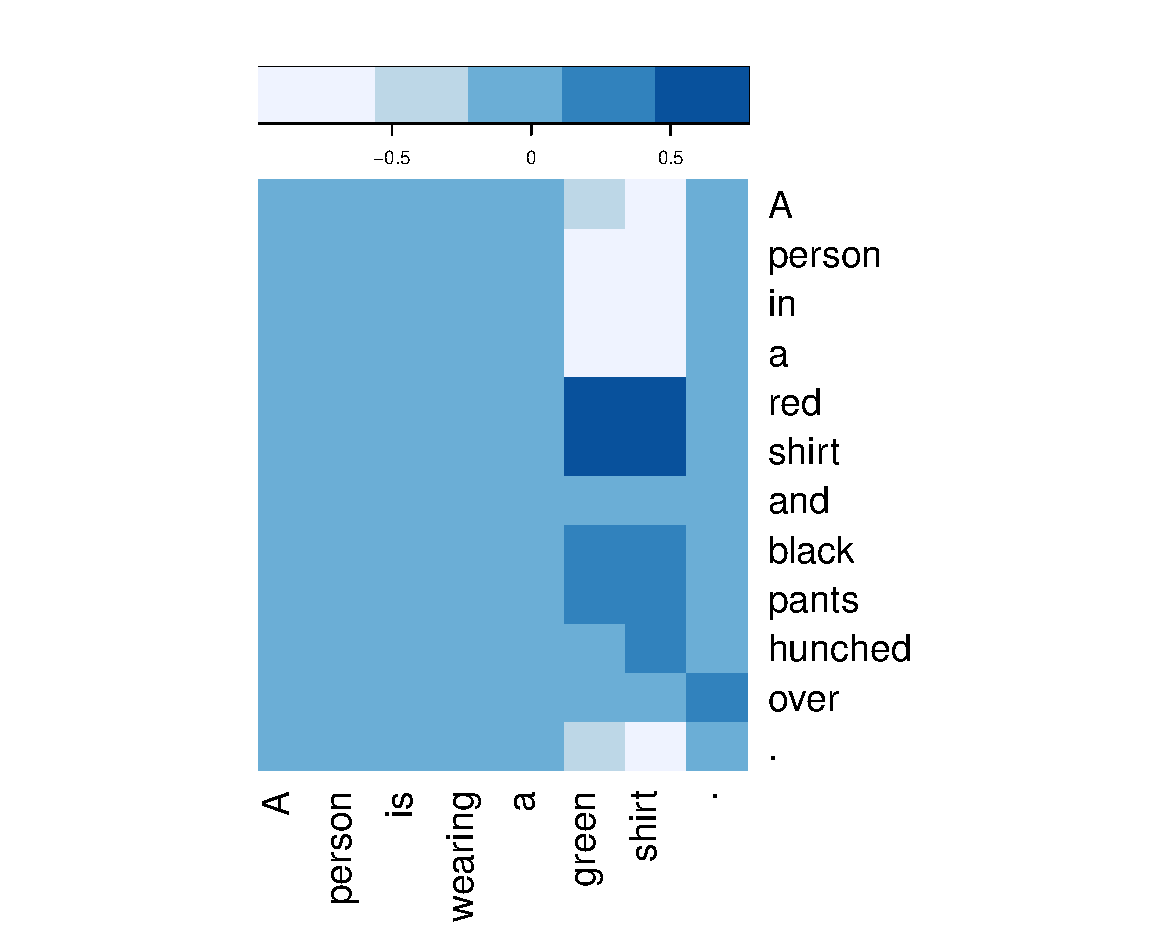
\includegraphics[height=5cm]{./fig/neuron17_case3.pdf}
  }\hspace{0.3cm}
  \subfloat[17th neuron]{
  %\includegraphics[width=0.45\linewidth]{./fig/lc-lstm.png}
  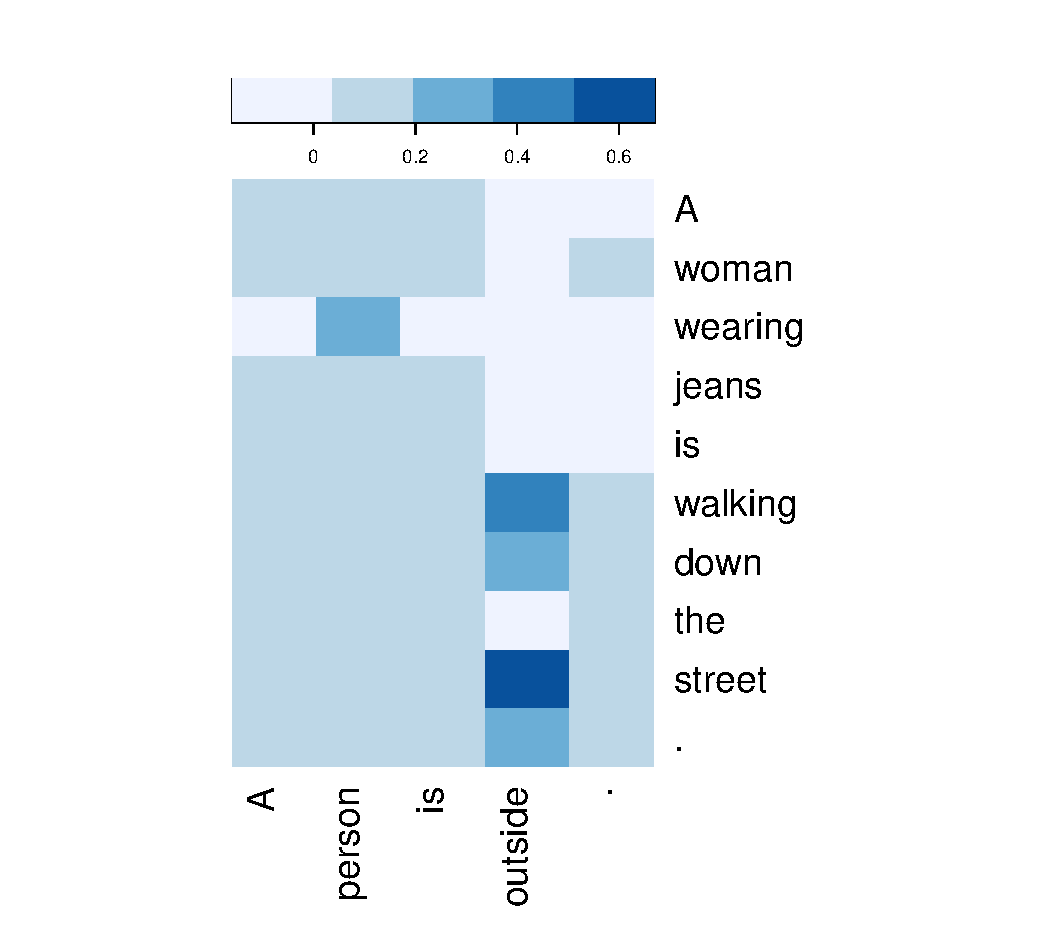
\includegraphics[height=5cm]{.//fig/neuron3_case1.pdf}
  }

  \caption{Illustration of two interpretable neurons and some word-pairs capture by these neurons. The darker patches denote the corresponding activations are higher.}\label{fig:case-studt}
\end{figure}


\subsubsection{Understanding Behaviors of Neurons in C-LSTMs}

To get an intuitive understanding of how the C-LSTMs work on this problem, we examined the neuron activations in the last aggregation layer while evaluating the test set using TC-LSTMs. We find that some cells are bound to certain roles.

%A surprising discovery is that the neurons in a certain position are playing a certain role. As shown in Fig. X, Neurons in Slice 17th can be activated once
%Each layer of neurons is bound to perform certain functions.

%A surprising discovery is that multiple interpretable cells do in fact exist in these networks.
%More precisely, given two sequences $X = x_1,x_2,\cdots,x_n$ and $Y = y_1,y_2,\cdots,y_m$, hidden state $\h_{i,j}$ can be emitted by C-LSTMs layer, where $n,m$ denote the lengths of two sequences.

%Let $\tilde{h}_{i,j,k}$ denote the maximum activation of $k_{th}$ neuron at the the point of $(i,j)$ for any $i \in \{1,\ldots,n\}$ and $j \in \{1,\ldots,m\}$, where $n,m$ denote the lengths of two sequences.


%Let $h_{i,j,k}$ denote the activation of $k_{th}$ neuron at the the point of $(i,j)$, which can obtains the maximum at $(\tilde{i}, \tilde{j})$ for any $i \in \{1,\ldots,n\}$ and $j \in \{1,\ldots,m\}$, where $n,m$ denote the lengths of two sequences.

Let $h_{i,j,k}$ denotes the activation of the $k$-th neuron at the position of $(i,j)$, where $i \in \{1,\ldots,n\}$ and $j \in \{1,\ldots,m\}$. By visualizing the hidden state $\h_{i,j,k}$ and analyzing the maximum activation, we can find that there exist multiple interpretable neurons.
For example, when some contextualized local perspectives are semantically related at point $({i},{j})$ of the sentence pair, the activation value of hidden neuron $h_{{i},{j},k}$ tend to be maximum, meaning that the model could capture some reasoning patterns.

Figure \ref{fig:case-studt} illustrates this phenomenon. In Figure \ref{fig:case-studt}(a), a neuron shows its ability to monitor the local contextual interactions about color.
The activation in the patch, including the word pair  ``\texttt{(red, green)}'', is much higher than others. This is informative pattern for the relation prediction of these two sentences, whose ground truth is contradiction. An interesting thing is there are two words describing color in the sentence `` \texttt{A person in a red shirt and black pants hunched over.}''. Our model ignores the useless word ``\texttt{black}'', which indicates that this neuron selectively captures pattern by contextual understanding, not just word level interaction.

In Figure \ref{fig:case-studt}(b), another neuron shows that it can capture the local contextual interactions, such as ``\texttt{(walking down the street, outside)}''. These patterns can be easily captured by pooling layer and provide a strong support for the final prediction.

Table \ref{tab:exp-pair} illustrates multiple interpretable neurons and some representative word or phrase pairs which can activate these neurons. %Here we just gives word pairs for better illustration.
These cases show that our models can capture contextual interactions beyond word level.


%说明哪些case受益于这个cell

%\textcolor[rgb]{1.00,0.00,0.00}{设计实验告诉review你是怎么发现这些现象的。}
%\begin{enumerate}
%  \item 可视化每个cell的tanh(c)
%  \item 给出统计结果,比如对于$17th$ cell, test data 中,colorful word-pair 一共出现过多少次,成功捕捉了多少次
%        对于$3nd$ cell, 所有gold 为entailment的句对中,该cell捕捉的word-pair 有多少是语义相关的;
%  \item 列个表,给出$3th$ cell 捕捉的word-pair.
%\end{enumerate}





%\begin{enumerate}
%  \item A woman wearing jeans is walking down the street .  A person is outside .
%  \item contradiction   contradiction   A bald man is getting out of a small blue car .     The bald man got out of a red truck .
%\end{enumerate}






%\paragraph{Performance comparisons}
%\paragraph{Errors eliminated by scaling up}


%
%The proposed attentive approach, ARC-III, provides an intuitive way to inspect the matching degree between the words in two sequences. This is done by visualizing the matching score $s_{ij}$ from Eq.\ref{eq:attention-1}.
%We sample two cases from paraphrase dataset, which are matched in test data.
%%As in Fig.\ref{fig:case-1},
%%The x-axis and y-axis of each plot correspond to the words in the two sequences from paraphrase dataset.
%
%From the Figure \ref{fig:case-1}-(a), we can see some important matching patters have been capture exactly, such as the phrase ``\texttt{left the courtroom}'' and ``\texttt{free man}''.  Besides, the model also finds some latent matching patterns
%such as the matching pair ``\texttt{(criminal charges, courtroom)}''. This may be due to the encoding of rereading information $c$ weighted by attention score.
%The right figure in Figure \ref{fig:case-1}-(b) also shows the effectiveness of our model. Some key matching pattern like ``\texttt{(equal,matched)}'' can be captured precisely.


\subsubsection{Error Analysis}
Although our models C-LSTMs are more sensitive to the discrepancy of the semantic capacity between two sentences, some semantic mistakes at the phrasal level still exist.
For example, our models failed to capture the key informative pattern when predicting the entailment sentence pair ``\texttt{A girl \textbf{takes off her shoes} and eats blue cotton candy/The girl is eating while \textbf{barefoot}.}''

Besides, despite the large size of the training corpus, it's still very different to solve some cases, which depend on the combination of the world knowledge and context-sensitive inferences.
For example, given an entailment pair ``\texttt{a man grabs his crotch during a political demonstration/The man is making a crude gesture}'', all models predict ``\texttt{neutral}''.
This analysis suggests that some architectural improvements or external world knowledge are necessary to eliminate all errors instead of simply scaling up the basic model.


\subsection{Experiment-II: Matching Question and Answer}
Matching question answering (MQA) is a typical task for semantic matching.
Given a question, we need select a correct answer from some candidate answers.

In this paper, we use the dataset collected  from Yahoo! Answers with the getByCategory function provided in Yahoo! Answers API, which produces $963,072$ questions and corresponding best answers. We then select the pairs in which the length of questions and answers are both in the interval $[4,30]$, thus obtaining $220,000$ question answer pairs to form the positive pairs.

For negative pairs, we first use each question's best answer as a query to retrieval top $1,000$ results from the whole answer set with Lucene, where $4$ or $9$ answers will be selected randomly to construct the negative pairs.

The whole dataset is divided into training, validation and testing data with proportion $20:1:1$. Moreover, we give two test settings: selecting the best answer from 5 and 10 candidates respectively.


\begin{table}[!t]\small
\center
\begin{tabular}{|l|*{4}{c|}}
\hline
\textbf{Model} & $k$  & P@1(5) & P@1(10) \\ \hline
Random Guess & - & 20.0 & 10.0 \\
NBOW & 50 &  63.9 & 47.6 \\
%single SRN & 50 &  64.9 & 49.3 \\
single LSTM  & 50 &  68.2 & 53.9 \\
parallel LSTMs & 50 &  66.9 & 52.1 \\
Attention LSTMs & 50 &  73.5 & 62.0 \\\hline
%Attention LSTM (w-by-w) & 50 &  - & - \\ \hline
LC-LSTMs (Single Direction) & 50 &  75.4 & 63.0 \\
LC-LSTMs & 50 &  76.1 & 64.1 \\
three stacked LC-LSTMs & 50 &  \textbf{78.5} & \textbf{66.2} \\ \hline

TC-LSTMs (Single Direction) & 50 &  74.3 & 62.4 \\
TC-LSTMs & 50 &  74.9 & 62.9 \\
three stacked TC-LSTMs & 50 &  77.0 & 65.3 \\ \hline
\end{tabular}
\caption{Results on Yahoo question-answer pairs dataset.}\label{tab:res-exp1}
\end{table}

\subsubsection{Results}
%Considering the codes of attention LSTMs and related models proposed by \cite{rocktaschel2015reasoning} have not been released,
Results of MQA are shown in the Table \ref{tab:res-exp1}. For our models,  due to stacking block more than three layers can not make significant improvements on this task, we just use three stacked C-LSTMs.

By analyzing the evaluation results of question-answer matching in table \ref{tab:res-exp1}, we can see
strong interaction models (attention LSTMs, our C-LSTMs) consistently outperform the weak interaction models (NBOW, parallel LSTMs) with a large margin, which suggests the importance of modelling strong interaction of two sentences.


Our proposed two C-LSTMs surpass the competitor methods and C-LSTMs augmented with multi-directions layers and multiple stacked blocks fully utilize multiple levels of abstraction to directly boost the performance.

Additionally, LC-LSTMs is superior to TC-LSTMs. The reason may be that MQA is a relative simple task, which requires less reasoning abilities, compared with RTE task. Moreover, the parameters of LC-LSTMs are less than TC-LSTMs, which ensures the former can avoid suffering from overfitting on a relatively smaller corpus.

%LC-LSTMs ensures the two sequences interact closely without being conflated thus more easily capturing local pattern of a sentence.



\section{Related Work}
Our architecture for sentence pair encoding can be regarded as strong interaction models, which have been explored in previous models.

An intuitive paradigm is to compute similarities between all the words or phrases of the two sentences. \newcite{socher2011dynamic} firstly used this paradigm for paraphrase detection. The representations of words or phrases are learned  based on recursive autoencoders. \newcite{wan2015deep} used LSTM to enhance the positional contextual interactions of the words or phrases between two sentences. The input of LSTM for one sentence does not involve another sentence.

A major limitation of this paradigm is the interaction of two sentence is captured by a pre-defined similarity measure. Thus, it is not easy to increase the depth of the network. Compared with this paradigm, we can stack our C-LSTMs to model multiple-granularity interactions of two sentences.

%\newcite{hu2014convolutional} proposed to a end-to-end architecture with convolutional neural network (Arc-II) to model multiple-granularity interactions of two sentences.

%Twhich   can be affected by another sentence
\newcite{rocktaschel2015reasoning} used two LSTMs equipped with attention mechanism to capture the iteration between two sentences. This architecture is asymmetrical for two sentences, where the obtained final representation is sensitive to the two sentences' order.

Compared with the attentive LSTM, our proposed C-LSTMs are symmetrical and model the local contextual interaction of two sequences directly.

%are capable of modelling more strong interactions, which  Unlike the methods of using similarity matrix, our method models the interaction of two sentences directly. Different with attention LSTMs, our models are symmetrical and the semantic interactions is captured by deep neural network.


%Our models are related to the long thread of work on sentence modelling, such as Neural Bag-of-Words (NBOW) model, recurrent neural network (RNN) \cite{mikolov2010recurrent,sutskever2014sequence,chung2014empirical}, recursive neural network (RecNN) \cite{socher2011parsing,socher2012semantic,socher2013recursive} and convolutional neural network (CNN) \cite{collobert2011natural,kalchbrenner2014convolutional,hu2014convolutional}. However these models are proposed for classification problems, our work relies heavily on a carefully designed attention mechanism.
%
%
%Another similar thread of work is the recent advances attention-based recurrent networks, which have been successfully applied to a wide variety of tasks machine translation\cite{bahdanau2014neural}, handwriting synthesis\cite{graves2013generating}, image caption generation\cite{xu2015show}.
%\newcite{hermann2015teaching} develops a class of attention based deep neural networks that learn to read real documents and answer complex questions, which are most related to our model. These models however do not apply attention mechanism to matching two sequences.
%In this paper, We introduce extensions to attention-based recurrent networks that make them applicable to match sequences.


%Aside from the models with recursive nature [15, 21, 19] (as discussed in Section 2.1), it is fairly common practice to use the sum of word-embedding to represent a short-text, mostly for classification [22]. There is very little work on convolutional modeling of language. In addition to [6, 18], there is a very recent model on sentence representation with dynamic convolutional neural network [9]. This work relies heavily on a carefully designed pooling strategy to handle the variable length of sentence with a relatively small feature map, tailored for classification problems with modest sizes.


\section{Conclusion and Future Work}
In this paper, we propose an end-to-end deep architecture to capture the strong interaction information of sentence pair. Experiments on two large scale text matching tasks demonstrate the efficacy of our proposed model and its superiority to competitor models.
Besides, our visualization analysis revealed that multiple interpretable neurons in our proposed models can capture the contextual interactions of the words or phrases.

In future work, we would like to incorporate some gating strategies into the depth dimension of our proposed models, like highway or residual network, to enhance the interactions between depth and other dimensions thus training more deep and powerful neural networks.

\bibliographystyle{named}
\bibliography{../nlp,../ours}

\end{document}
